% These are the lecture notes for my CSCI360 course SPRING 2017
% at John Jay College of Criminal Justice. They are based largely on
% Schneier's Applied Cryptography.

% Feel free to edit these slides and use them for your own courses.
% HOWEVER DO NOT REMOVE THESE LINES!
% Email me at: awood [at] jjay.cuny.edu
% or at: awood [at] gradcenter.cuny.edu


\documentclass{beamer}

\usepackage{tikz}
\usetikzlibrary{calc}

\usepackage{forest}
\usepackage{verbatim}
\usepackage{color}
\usepackage{amsmath}


\setbeamertemplate{footline}[frame number]
\setbeamertemplate{navigation symbols}{} 

\newtheorem{thm}{Theorem}[section]
\newtheorem{lem}{Lemma}
\newtheorem{cl}{Claim}
\newtheorem{cor}{Corollary}[section]
\newtheorem{conj}{Conjecture}
\newtheorem{quest}{Question}
\newtheorem{defn}{Definition}[section]
\newtheorem{obs}{Observation}[section]
\newtheorem{exam}{Example}

\newcommand{\im}{\operatorname{im}}
\newcommand{\id}{\operatorname{id}}
\newcommand{\interior}{\operatorname{int}}
\newcommand{\bdry}{\operatorname{bdry}}
\newcommand{\<}{\langle}
\renewcommand{\>}{\rangle}
\newcommand{\Gab}{(G_\phi)^{ab}} 
\newcommand{\phibar}{\bar{\phi}}
\newcommand{\Z}{\mathbb{Z}}
\newcommand{\N}{\mathbb{N}}
\newcommand{\Q}{\mathbb{Q}}
\newcommand{\R}{\mathbb{R}}
\newcommand{\C}{\mathbb{C}}
\newcommand{\A}{\mathcal{A}}
\newcommand{\OO}{\mathcal{O}}
\newcommand{\UU}{\mathcal{U}}
\newcommand{\power}{2^{\{P_1, \cdots , P_n\}}}
\newcommand{\bp}{\begin{problem}}
\newcommand{\ep}{\end{problem}}
\newcommand{\ba}{\begin{answer}}
\newcommand{\ea}{\end{answer}}
\newcommand{\ds}{\displaystyle}
\newcommand{\ben}{\renewcommand{\theenumi}{\alph{enumi}}
\renewcommand{\labelenumi}{(\theenumi)}\begin{enumerate}}
\newcommand{\een}{\end{enumerate}}
\newcommand{\Hess}{\operatorname{Hessian}}
\newcommand{\Aut}{\mathrm{Aut}}
\newcommand{\Inn}{\mathrm{Inn}}
\newcommand{\Out}{\mathrm{Out}}
\newcommand{\End}{\mathrm{End}}


\mode<presentation>
{
%  \usetheme{default}
  \setbeamercovered{invisible}
}


\usepackage[english]{babel}
\usepackage[latin1]{inputenc}
\usepackage{times}
\usepackage[T1]{fontenc}
\usepackage{stmaryrd}

%\usetheme{default}
%\usetheme{AnnArbor}
%\usetheme{Antibes}
%\usetheme{Bergen}
%\usetheme{Berkeley}
%\usetheme{Berlin}
%\usetheme{Boadilla}
%\usetheme{CambridgeUS}
%\usetheme{Copenhagen}
%\usetheme{Darmstadt}
%\usetheme{Dresden}
%\usetheme{Frankfurt}
%\usetheme{Goettingen}
%\usetheme{Hannover}
%\usetheme{Ilmenau}
%\usetheme{JuanLesPins}
%\usetheme{Luebeck}
%\usetheme{Madrid}
%\usetheme{Malmoe}
%\usetheme{Marburg}
%\usetheme{Montpellier}
%\usetheme{PaloAlto}
%\usetheme{Pittsburgh}
%\usetheme{Rochester}
\usetheme{Singapore}
%\usetheme{Szeged}
%\usetheme{Warsaw}

%\usecolortheme{default}
%\usecolortheme{albatross}
\usecolortheme{beaver}
%\usecolortheme{beetle}
%\usecolortheme{crane}
%\usecolortheme{dolphin}
%\usecolortheme{dove} % grey, white, yellow
%\usecolortheme{fly} %grey, yellow
%\usecolortheme{lily} %white, yellow, blue
%\usecolortheme{orchid}
%\usecolortheme{rose}
%\usecolortheme{seagull}
%\usecolortheme{seahorse}
%\usecolortheme{whale}
%\usecolortheme{wolverine}

% Title page

\title[Block Ciphers]{Block Ciphers}

\subtitle{Based on \emph{Cryptography Engineering} sections 3.3, 3.4 \\ By Ferguson, Schnier, and Kohno}

\author
{Lecture notes of Alexander Wood \\ \scriptsize \href{mailto:awood@jjay.cuny.edu}{awood@jjay.cuny.edu}}
\institute[JJay]{John Jay College of Criminal Justice}  

\date{}

\begin{document}

% Remove 'figure' text from figure captions 
\setbeamertemplate{caption}{\raggedright\insertcaption\par}

\begin{frame}
  \titlepage
\end{frame}

\section{Overview}


\begin{frame}
\frametitle{What is a block?}

A \textbf{block} is a chuck of data of a predetermined size. For instance a block of $64$ contiguous bits.  \newline

When encrypting with blocks, we encrypt data block-by-block.
\end{frame}


\begin{frame}
\frametitle{Block Encryption}

\begin{figure}
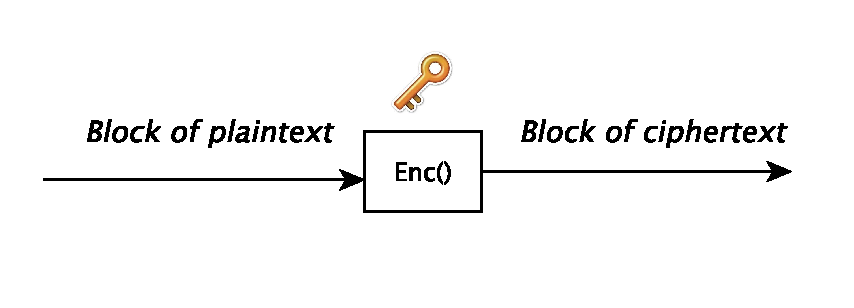
\includegraphics[scale=.6]{IMG/blockencrypt.pdf}
\end{figure}
Identical blocks should be encrypted to different ciphertexts! To do this we must introduce a notion of \textbf{randomness}, one of the most important concepts in cryptography. 
\end{frame}

\begin{frame}
\frametitle{Block Size: Not Too Small!}

With a bit block of size $L$ there are $2^L$ possible plaintext bit combinations. A larger block size means there are more possible plaintext bits. Thus we wish to \textbf{avoid very small blocks}. 
\end{frame}


\begin{frame}
\frametitle{Block Size: Not Too Large!}
A block size too large makes the ciphertext too inefficient to work with. \textbf{Avoid very large blocks}. 
\end{frame}


\begin{frame}
\frametitle{Block Size: Just Right!}

Preferred block sizes are \textbf{multiples of 8} since most processors handle data in multiples of 8 (ie, the length of a byte).
\end{frame}


\begin{frame}
\frametitle{Padding a Block Cipher}

When a plaintext is shorter than the desired block size it is \textbf{padded} with redundant information, making the last block the necessary block size. \newline

Padding should be randomized each time it is applied. Too much padding can make the system inefficient. (Hence, the need to avoid too large of a block size!)
\end{frame}

\begin{frame}
\frametitle{Block Cipher Schemes}

\begin{itemize}
\item {\color{red}\textbf{Digital Encryption Standard (DES)}} {\scriptsize $\leftarrow$ Next class!}
\item Triple DES
\item Advanced Encryption Standard (AES)
\item IDEA
\item Twofish
\item Serpent
\end{itemize}
\end{frame}

\section{Theory}

\begin{frame}
\frametitle{What is block cipher security?}

\begin{figure}
\includegraphics[scale=.3]{IMG/confused.jpg}
\end{figure}\centering
???
\end{frame}


\begin{frame}
\frametitle{What is block cipher security?}

It's difficult to formalize! We give a ``sketch'' of the definition in these slides.
\end{frame}


\begin{frame}
\frametitle{Ideal Block Ciphers}

We define block cipher security in relation to an \textbf{ideal block cipher}. An ideal block cipher is a random permutation, meaning:
\begin{itemize}
\item For each key, the block cipher is a \textbf{random} permutation
\item The key-permutation pairs shold be chosen \textbf{randomly}
\end{itemize}
\end{frame}


\begin{frame}
\frametitle{Ideal Block Ciphers}

A more formal definition would introduce a \textbf{uniform probability distribution} over the set of all \emph{possible} block ciphers. 
\end{frame}


\section{Security}
\begin{frame}
\frametitle{Block Cipher Security (Informal Definition)}

A block cipher is \textbf{secure} if no attack against it exists.
\end{frame}


\begin{frame}
\frametitle{Block Cipher Security (Informal Definition)}

Okay.. but what does this mean?

\begin{figure}
\includegraphics[scale=.5]{IMG/confused2}
\end{figure}
\end{frame}

\begin{frame}
\frametitle{Attack Against A Block Cipher}

A method of distinguishing between a given block cipher and an ideal block cipher is called an \textbf{attack} on the given block cipher. 
\end{frame}


\begin{frame}
\frametitle{Okay.. but what does ``distinguishing'' mean?}

\begin{figure}
\includegraphics[scale=.5]{IMG/confused3}
\end{figure}
\end{frame}


\section{Distinguishers}
\begin{frame}
\frametitle{Distinguishers}

A \textbf{distinguisher} is a black-box function which provides means to compare a given block cipher to the ``ideal'' construct of a block cipher. \newline
\end{frame}


\begin{frame}
\frametitle{Distinguishers}

\begin{figure}
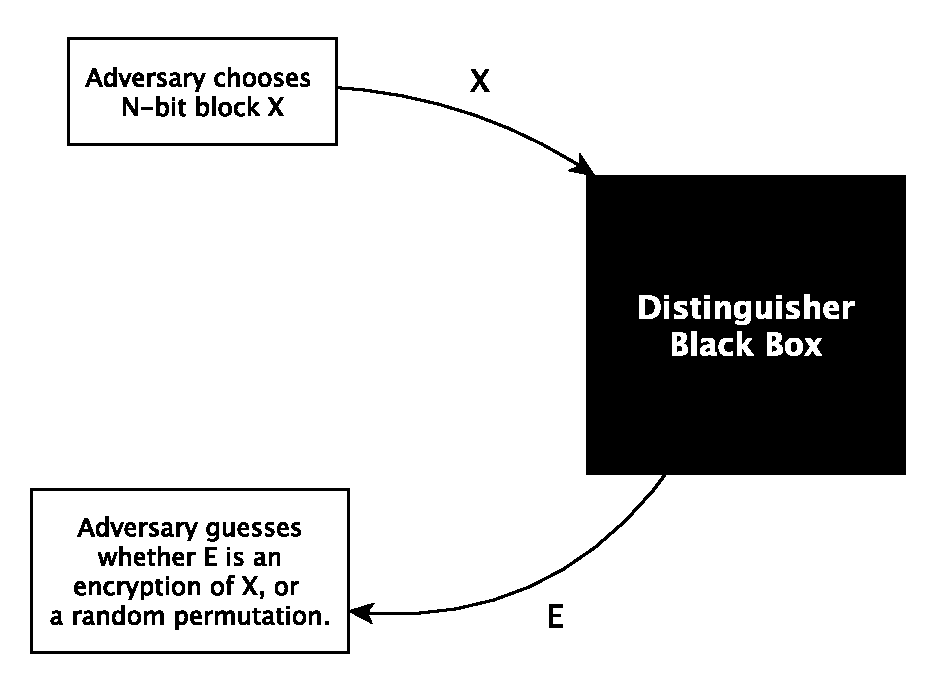
\includegraphics[scale=.5]{IMG/blackboxdist}
\end{figure}
\end{frame}

\begin{frame}
\frametitle{Computational Distinguishability}

There are various types of indistinguishability. In Cryptography we often look at \textbf{computational indistinguishability} -- given a certain amount of computational resources, can the distinguisher function tell the difference between the given scenario and the ideal scenario?
\end{frame}


\begin{frame}
\frametitle{Distinguishers}

The distinguisher is a theoretical model. It has access to both the encryption, decryption, and key generation functions. It is free to choose any key during its operations. \newline

The adversary does \emph{not} know whether the black box is implementing the block cipher or the ideal block cipher. \newline

The job of the adversary is to determine whether the ideal or the given block cipher is being implemented by the black box function.
\end{frame}

\begin{frame}
\frametitle{Distinguishers}

Note that the adversary does not have to get it right every time! It only has to get it right more often than not. \newline

This means that with a probability more than negligibly greater than $50\%$, the adversary can tell you whether the black box is running with the given block cipher or with an ideal block cipher. 
\end{frame}


\begin{frame}[fragile]
\frametitle{Distinguisher Game}

Let $E$ be an $n$-bit block cipher and $D$ a distinguisher.
\begin{itemize}
\item $D$ randomly chooses a bit $0$ or $1$.
\item  The attacker chooses an $n$-bit block $X$ and sends it to the distinguisher.
\item  The distinguisher $D$ carries out the following:
	\begin{itemize}
	\item If $D$ chose $0$, then $D$ chooses a random key $K$ and will output \verb|Enc|$_k(X)$.
	\item If $D$ chose $1$, then $D$ will output a random permutation of length $n$.
	\end{itemize}
\item Step $2$ is repeated $q$ times.
\item The attack guesses the bit $0$ or $1$ and wins if the guess is correct. 
\end{itemize}
\end{frame}


\begin{frame}
\frametitle{Distinguisher Game}

\begin{figure}
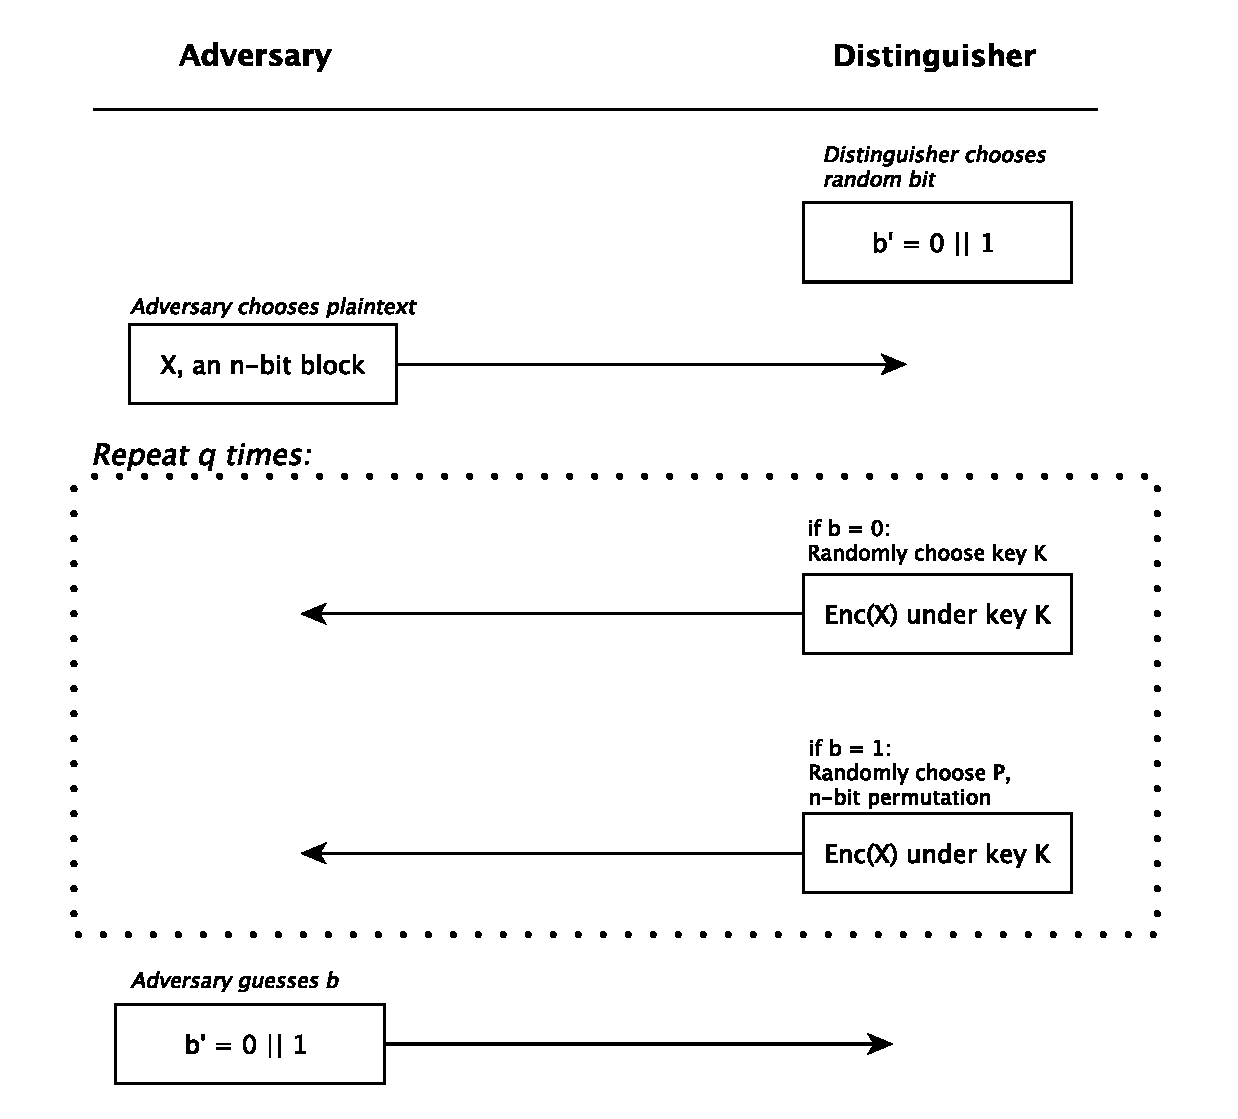
\includegraphics[scale=.4]{IMG/game}
\end{figure}
\end{frame}

\begin{frame}
\frametitle{Example 1: A Trivial Distinguisher}

Encrypt the plaintext $0$ with the key $0$. See if the result matches what we expect from a block cipher $X$.\newline

This is called \emph{trivial}, or \emph{generic}. When looking at block cipher security we need to look at \emph{non-generic} cases.
\end{frame}


\section{Genericity}
\begin{frame}
\frametitle{What is non-generic}

The book explains: ``it's a bit like an obscenity: we know it when we see it.''
\end{frame}

\begin{frame}
\frametitle{What is non-generic?}

We can do a bit better than that. \newline

The generic attack above is so simple that we could even use it to distinguish between two ideal block ciphers. \newline

We want an attack that exploits the internal properties of the block themselves.
\end{frame}


\begin{frame}
\frametitle{Example 2: More Complicated, But Generic}

Encrypt the plaintext $0$ with all keys in the range $1, \dots, 2^{32}$. Count how often each value for the first $32$ bits of ciphertext occurs. \newline

If a value repeats $5$ times, instead of the expected $1$ time which would happen with a random block, then we have found a property which is unlikely to hold for an ideal block.
\end{frame}


\begin{frame}
\frametitle{Example 2: More Complicated, But Generic}

However this distinguisher is still generic! It is still applicable to \emph{all} block ciphers and does not use the properties of the \emph{given} block cipher $X$.
\end{frame}


\begin{frame}
\frametitle{Example 3: Non-Generic Distinguisher}

\begin{enumerate}
\item Make a list of 1000 different statistics you can compute about a given cipher.
\item Compute \emph{each} of these for a given block $X$.
\item Build the distinguisher from the statistic which gives the most significant result.
\end{enumerate}
\end{frame}

\begin{frame}
\frametitle{Example 3: Non-Generic Distinguisher}

We expect to find a statistic with a significance level of 1 in 1000.  \newline

This distinguisher can be applied to any individual cipher hence it is non-generic. 
\end{frame}


\begin{frame}
\frametitle{Computational Indistinguishability of Block Ciphers}

What we are looking for usually is not perfect indistinguishability -- it is only \textbf{computational indistinguishability}. We wish to be unable to distinguish between a block $X$ and an ideal block cipher given a predetermined amount of limited computational resources. 
\end{frame}


\begin{frame}
\frametitle{References}

\begin{itemize}
\item \url{https://www.tutorialspoint.com/cryptography/block_cipher.htm}
\item \emph{Cryptography Engineering} sections 3.3, 3.4 \\ By Ferguson, Schnier, and Kohno
\end{itemize}
\end{frame}
\end{document}


